\documentclass[twoside]{book}

% Packages required by doxygen
\usepackage{fixltx2e}
\usepackage{calc}
\usepackage{doxygen}
\usepackage[export]{adjustbox} % also loads graphicx
\usepackage{graphicx}
\usepackage[utf8]{inputenc}
\usepackage{makeidx}
\usepackage{multicol}
\usepackage{multirow}
\PassOptionsToPackage{warn}{textcomp}
\usepackage{textcomp}
\usepackage[nointegrals]{wasysym}
\usepackage[table]{xcolor}

% Font selection
\usepackage[T1]{fontenc}
\usepackage[scaled=.90]{helvet}
\usepackage{courier}
\usepackage{amssymb}
\usepackage{sectsty}
\renewcommand{\familydefault}{\sfdefault}
\allsectionsfont{%
  \fontseries{bc}\selectfont%
  \color{darkgray}%
}
\renewcommand{\DoxyLabelFont}{%
  \fontseries{bc}\selectfont%
  \color{darkgray}%
}
\newcommand{\+}{\discretionary{\mbox{\scriptsize$\hookleftarrow$}}{}{}}

% Page & text layout
\usepackage{geometry}
\geometry{%
  a4paper,%
  top=2.5cm,%
  bottom=2.5cm,%
  left=2.5cm,%
  right=2.5cm%
}
\tolerance=750
\hfuzz=15pt
\hbadness=750
\setlength{\emergencystretch}{15pt}
\setlength{\parindent}{0cm}
\setlength{\parskip}{3ex plus 2ex minus 2ex}
\makeatletter
\renewcommand{\paragraph}{%
  \@startsection{paragraph}{4}{0ex}{-1.0ex}{1.0ex}{%
    \normalfont\normalsize\bfseries\SS@parafont%
  }%
}
\renewcommand{\subparagraph}{%
  \@startsection{subparagraph}{5}{0ex}{-1.0ex}{1.0ex}{%
    \normalfont\normalsize\bfseries\SS@subparafont%
  }%
}
\makeatother

% Headers & footers
\usepackage{fancyhdr}
\pagestyle{fancyplain}
\fancyhead[LE]{\fancyplain{}{\bfseries\thepage}}
\fancyhead[CE]{\fancyplain{}{}}
\fancyhead[RE]{\fancyplain{}{\bfseries\leftmark}}
\fancyhead[LO]{\fancyplain{}{\bfseries\rightmark}}
\fancyhead[CO]{\fancyplain{}{}}
\fancyhead[RO]{\fancyplain{}{\bfseries\thepage}}
\fancyfoot[LE]{\fancyplain{}{}}
\fancyfoot[CE]{\fancyplain{}{}}
\fancyfoot[RE]{\fancyplain{}{\bfseries\scriptsize Generated by Doxygen }}
\fancyfoot[LO]{\fancyplain{}{\bfseries\scriptsize Generated by Doxygen }}
\fancyfoot[CO]{\fancyplain{}{}}
\fancyfoot[RO]{\fancyplain{}{}}
\renewcommand{\footrulewidth}{0.4pt}
\renewcommand{\chaptermark}[1]{%
  \markboth{#1}{}%
}
\renewcommand{\sectionmark}[1]{%
  \markright{\thesection\ #1}%
}

% Indices & bibliography
\usepackage{natbib}
\usepackage[titles]{tocloft}
\setcounter{tocdepth}{3}
\setcounter{secnumdepth}{5}
\makeindex

% Hyperlinks (required, but should be loaded last)
\usepackage{ifpdf}
\ifpdf
  \usepackage[pdftex,pagebackref=true]{hyperref}
\else
  \usepackage[ps2pdf,pagebackref=true]{hyperref}
\fi
\hypersetup{%
  colorlinks=true,%
  linkcolor=blue,%
  citecolor=blue,%
  unicode%
}

% Custom commands
\newcommand{\clearemptydoublepage}{%
  \newpage{\pagestyle{empty}\cleardoublepage}%
}

\usepackage{caption}
\captionsetup{labelsep=space,justification=centering,font={bf},singlelinecheck=off,skip=4pt,position=top}

%===== C O N T E N T S =====

\begin{document}

% Titlepage & ToC
\hypersetup{pageanchor=false,
             bookmarksnumbered=true,
             pdfencoding=unicode
            }
\pagenumbering{roman}
\begin{titlepage}
\vspace*{7cm}
\begin{center}%
{\Large Y\+D\+L\+I\+D\+AR A\+R\+D\+U\+I\+NO }\\
\vspace*{1cm}
{\large Generated by Doxygen 1.8.11}\\
\end{center}
\end{titlepage}
\clearemptydoublepage
\tableofcontents
\clearemptydoublepage
\pagenumbering{arabic}
\hypersetup{pageanchor=true}

%--- Begin generated contents ---
\chapter{Class Index}
\section{Class List}
Here are the classes, structs, unions and interfaces with brief descriptions\+:\begin{DoxyCompactList}
\item\contentsline{section}{\hyperlink{structcmd__packet}{cmd\+\_\+packet} }{\pageref{structcmd__packet}}{}
\item\contentsline{section}{\hyperlink{structdevice__health}{device\+\_\+health} }{\pageref{structdevice__health}}{}
\item\contentsline{section}{\hyperlink{structdevice__info}{device\+\_\+info} }{\pageref{structdevice__info}}{}
\item\contentsline{section}{\hyperlink{structlidar__ans__header}{lidar\+\_\+ans\+\_\+header} }{\pageref{structlidar__ans__header}}{}
\item\contentsline{section}{\hyperlink{structnode__info}{node\+\_\+info} }{\pageref{structnode__info}}{}
\item\contentsline{section}{\hyperlink{structnode__package}{node\+\_\+package} }{\pageref{structnode__package}}{}
\item\contentsline{section}{\hyperlink{class_queue_list}{Queue\+List$<$ T $>$} }{\pageref{class_queue_list}}{}
\item\contentsline{section}{\hyperlink{structsampling__rate}{sampling\+\_\+rate} }{\pageref{structsampling__rate}}{}
\item\contentsline{section}{\hyperlink{structscan__frequency}{scan\+\_\+frequency} }{\pageref{structscan__frequency}}{}
\item\contentsline{section}{\hyperlink{structscan__rotation}{scan\+\_\+rotation} }{\pageref{structscan__rotation}}{}
\item\contentsline{section}{\hyperlink{structscan_point}{scan\+Point} }{\pageref{structscan_point}}{}
\item\contentsline{section}{\hyperlink{class_y_d_lidar}{Y\+D\+Lidar} }{\pageref{class_y_d_lidar}}{}
\end{DoxyCompactList}

\chapter{Class Documentation}
\hypertarget{structcmd__packet}{}\section{cmd\+\_\+packet Struct Reference}
\label{structcmd__packet}\index{cmd\+\_\+packet@{cmd\+\_\+packet}}
\subsection*{Public Attributes}
\begin{DoxyCompactItemize}
\item 
uint8\+\_\+t {\bfseries sync\+Byte}\hypertarget{structcmd__packet_afbbf12329459d281e93fc742d1a78009}{}\label{structcmd__packet_afbbf12329459d281e93fc742d1a78009}

\item 
uint8\+\_\+t {\bfseries cmd\+\_\+flag}\hypertarget{structcmd__packet_a87508f8232c382897c9159026985f3eb}{}\label{structcmd__packet_a87508f8232c382897c9159026985f3eb}

\item 
uint8\+\_\+t {\bfseries size}\hypertarget{structcmd__packet_aff384923e9d1d54d526ca755529eac05}{}\label{structcmd__packet_aff384923e9d1d54d526ca755529eac05}

\item 
uint8\+\_\+t {\bfseries data}\hypertarget{structcmd__packet_a3b8820a6357e147dd00ea67d9c9484c0}{}\label{structcmd__packet_a3b8820a6357e147dd00ea67d9c9484c0}

\end{DoxyCompactItemize}


The documentation for this struct was generated from the following file\+:\begin{DoxyCompactItemize}
\item 
Y\+D\+Lidar.\+h\end{DoxyCompactItemize}

\hypertarget{structdevice__health}{}\section{device\+\_\+health Struct Reference}
\label{structdevice__health}\index{device\+\_\+health@{device\+\_\+health}}
\subsection*{Public Attributes}
\begin{DoxyCompactItemize}
\item 
uint8\+\_\+t {\bfseries status}\hypertarget{structdevice__health_ac3425f5555ecbb5a0da03b4cabe2777c}{}\label{structdevice__health_ac3425f5555ecbb5a0da03b4cabe2777c}

\item 
uint16\+\_\+t {\bfseries error\+\_\+code}\hypertarget{structdevice__health_a8815828d6de33cb43e8b72da48f51f23}{}\label{structdevice__health_a8815828d6de33cb43e8b72da48f51f23}

\end{DoxyCompactItemize}


The documentation for this struct was generated from the following file\+:\begin{DoxyCompactItemize}
\item 
Y\+D\+Lidar.\+h\end{DoxyCompactItemize}

\hypertarget{structdevice__info}{}\section{device\+\_\+info Struct Reference}
\label{structdevice__info}\index{device\+\_\+info@{device\+\_\+info}}
\subsection*{Public Attributes}
\begin{DoxyCompactItemize}
\item 
uint8\+\_\+t {\bfseries model}\hypertarget{structdevice__info_a3c491b342ed11af3c70358e7e8f6c935}{}\label{structdevice__info_a3c491b342ed11af3c70358e7e8f6c935}

\item 
uint16\+\_\+t {\bfseries firmware\+\_\+version}\hypertarget{structdevice__info_af3d369a410577d85ec6b59ffeeaade48}{}\label{structdevice__info_af3d369a410577d85ec6b59ffeeaade48}

\item 
uint8\+\_\+t {\bfseries hardware\+\_\+version}\hypertarget{structdevice__info_add77e9b0edbc4a0dbd8f91b0cac9ea13}{}\label{structdevice__info_add77e9b0edbc4a0dbd8f91b0cac9ea13}

\item 
uint8\+\_\+t {\bfseries serialnum} \mbox{[}16\mbox{]}\hypertarget{structdevice__info_abf23e35480aff36d846085ca6fd0eec3}{}\label{structdevice__info_abf23e35480aff36d846085ca6fd0eec3}

\end{DoxyCompactItemize}


The documentation for this struct was generated from the following file\+:\begin{DoxyCompactItemize}
\item 
Y\+D\+Lidar.\+h\end{DoxyCompactItemize}

\hypertarget{structlidar__ans__header}{}\section{lidar\+\_\+ans\+\_\+header Struct Reference}
\label{structlidar__ans__header}\index{lidar\+\_\+ans\+\_\+header@{lidar\+\_\+ans\+\_\+header}}
\subsection*{Public Attributes}
\begin{DoxyCompactItemize}
\item 
uint8\+\_\+t {\bfseries sync\+Byte1}\hypertarget{structlidar__ans__header_aeaa5beb7182c922d6d68697ecf60318a}{}\label{structlidar__ans__header_aeaa5beb7182c922d6d68697ecf60318a}

\item 
uint8\+\_\+t {\bfseries sync\+Byte2}\hypertarget{structlidar__ans__header_a9ce80818478513e1cb36de5a17917958}{}\label{structlidar__ans__header_a9ce80818478513e1cb36de5a17917958}

\item 
uint32\+\_\+t {\bfseries size}\+:30\hypertarget{structlidar__ans__header_a6e01bc2ec02153e40f3402790b917af3}{}\label{structlidar__ans__header_a6e01bc2ec02153e40f3402790b917af3}

\item 
uint32\+\_\+t {\bfseries sub\+Type}\+:2\hypertarget{structlidar__ans__header_abd31cd42537cebe7958b95d3f4a07169}{}\label{structlidar__ans__header_abd31cd42537cebe7958b95d3f4a07169}

\item 
uint8\+\_\+t {\bfseries type}\hypertarget{structlidar__ans__header_aab38102a1a266b5bfb842b10bf2804b2}{}\label{structlidar__ans__header_aab38102a1a266b5bfb842b10bf2804b2}

\end{DoxyCompactItemize}


The documentation for this struct was generated from the following file\+:\begin{DoxyCompactItemize}
\item 
Y\+D\+Lidar.\+h\end{DoxyCompactItemize}

\hypertarget{structnode__info}{}\section{node\+\_\+info Struct Reference}
\label{structnode__info}\index{node\+\_\+info@{node\+\_\+info}}
\subsection*{Public Attributes}
\begin{DoxyCompactItemize}
\item 
uint8\+\_\+t {\bfseries sync\+\_\+quality}\hypertarget{structnode__info_a45f5ed4efbe416d43171d63c669f02da}{}\label{structnode__info_a45f5ed4efbe416d43171d63c669f02da}

\item 
uint16\+\_\+t {\bfseries angle\+\_\+q6\+\_\+checkbit}\hypertarget{structnode__info_a73e1d282a573f3daa74332fe29b90a26}{}\label{structnode__info_a73e1d282a573f3daa74332fe29b90a26}

\item 
uint16\+\_\+t {\bfseries distance\+\_\+q2}\hypertarget{structnode__info_a82eaf27a6196e803d3618c83b052f78c}{}\label{structnode__info_a82eaf27a6196e803d3618c83b052f78c}

\end{DoxyCompactItemize}


The documentation for this struct was generated from the following file\+:\begin{DoxyCompactItemize}
\item 
Y\+D\+Lidar.\+h\end{DoxyCompactItemize}

\hypertarget{structnode__package}{}\section{node\+\_\+package Struct Reference}
\label{structnode__package}\index{node\+\_\+package@{node\+\_\+package}}
\subsection*{Public Attributes}
\begin{DoxyCompactItemize}
\item 
uint16\+\_\+t {\bfseries package\+\_\+\+Head}\hypertarget{structnode__package_a6d48d3a1d1ef718065a82e7495fa2b26}{}\label{structnode__package_a6d48d3a1d1ef718065a82e7495fa2b26}

\item 
uint8\+\_\+t {\bfseries package\+\_\+\+CT}\hypertarget{structnode__package_a3be7b81a7cc4b7ef7beb816ccd414579}{}\label{structnode__package_a3be7b81a7cc4b7ef7beb816ccd414579}

\item 
uint8\+\_\+t {\bfseries now\+Package\+Num}\hypertarget{structnode__package_aad0a75920ad5c1393f1b00904ece2d67}{}\label{structnode__package_aad0a75920ad5c1393f1b00904ece2d67}

\item 
uint16\+\_\+t {\bfseries package\+First\+Sample\+Angle}\hypertarget{structnode__package_ac224f6450e8bd5bd069149babc37e1c4}{}\label{structnode__package_ac224f6450e8bd5bd069149babc37e1c4}

\item 
uint16\+\_\+t {\bfseries package\+Last\+Sample\+Angle}\hypertarget{structnode__package_af5768e03270d3b7d7f58b3b82156dc2e}{}\label{structnode__package_af5768e03270d3b7d7f58b3b82156dc2e}

\item 
uint16\+\_\+t {\bfseries check\+Sum}\hypertarget{structnode__package_a4b6d9990da9343143161aae929bb986e}{}\label{structnode__package_a4b6d9990da9343143161aae929bb986e}

\item 
uint16\+\_\+t {\bfseries package\+Sample\+Distance} \mbox{[}Package\+Sample\+Max\+Lngth\mbox{]}\hypertarget{structnode__package_a00ee27fc439bd21ed97ee20fe7febdc9}{}\label{structnode__package_a00ee27fc439bd21ed97ee20fe7febdc9}

\end{DoxyCompactItemize}


The documentation for this struct was generated from the following file\+:\begin{DoxyCompactItemize}
\item 
Y\+D\+Lidar.\+h\end{DoxyCompactItemize}

\hypertarget{class_queue_list}{}\section{Queue\+List$<$ T $>$ Class Template Reference}
\label{class_queue_list}\index{Queue\+List$<$ T $>$@{Queue\+List$<$ T $>$}}
\subsection*{Public Member Functions}
\begin{DoxyCompactItemize}
\item 
void {\bfseries push} (const T i)\hypertarget{class_queue_list_a47c26444335b418138450ba8bfb5ba13}{}\label{class_queue_list_a47c26444335b418138450ba8bfb5ba13}

\item 
T {\bfseries pop} ()\hypertarget{class_queue_list_abf5fba15da77e79d28cb3f593f5fd0a7}{}\label{class_queue_list_abf5fba15da77e79d28cb3f593f5fd0a7}

\item 
T {\bfseries peek} () const \hypertarget{class_queue_list_aed5225e36fcedf948a08d8c6b856be9f}{}\label{class_queue_list_aed5225e36fcedf948a08d8c6b856be9f}

\item 
bool {\bfseries is\+Empty} () const \hypertarget{class_queue_list_ab6c04bc7c2b54ac9060f8a0f1b738351}{}\label{class_queue_list_ab6c04bc7c2b54ac9060f8a0f1b738351}

\item 
int {\bfseries count} () const \hypertarget{class_queue_list_a078a1e9b8021ea45c9b1110d09602ef9}{}\label{class_queue_list_a078a1e9b8021ea45c9b1110d09602ef9}

\end{DoxyCompactItemize}


The documentation for this class was generated from the following file\+:\begin{DoxyCompactItemize}
\item 
examples/\+Y\+D\+Lidar\+\_\+\+Serial\+Event/Queue\+List.\+h\end{DoxyCompactItemize}

\hypertarget{structsampling__rate}{}\section{sampling\+\_\+rate Struct Reference}
\label{structsampling__rate}\index{sampling\+\_\+rate@{sampling\+\_\+rate}}
\subsection*{Public Attributes}
\begin{DoxyCompactItemize}
\item 
uint8\+\_\+t {\bfseries rate}\hypertarget{structsampling__rate_a8d860fbedd930d2022fe7bb6cf1f78b6}{}\label{structsampling__rate_a8d860fbedd930d2022fe7bb6cf1f78b6}

\end{DoxyCompactItemize}


The documentation for this struct was generated from the following file\+:\begin{DoxyCompactItemize}
\item 
Y\+D\+Lidar.\+h\end{DoxyCompactItemize}

\hypertarget{structscan__frequency}{}\section{scan\+\_\+frequency Struct Reference}
\label{structscan__frequency}\index{scan\+\_\+frequency@{scan\+\_\+frequency}}
\subsection*{Public Attributes}
\begin{DoxyCompactItemize}
\item 
uint32\+\_\+t {\bfseries frequency}\hypertarget{structscan__frequency_ae4f2152e77416cff02f44452355f2808}{}\label{structscan__frequency_ae4f2152e77416cff02f44452355f2808}

\end{DoxyCompactItemize}


The documentation for this struct was generated from the following file\+:\begin{DoxyCompactItemize}
\item 
Y\+D\+Lidar.\+h\end{DoxyCompactItemize}

\hypertarget{structscan__rotation}{}\section{scan\+\_\+rotation Struct Reference}
\label{structscan__rotation}\index{scan\+\_\+rotation@{scan\+\_\+rotation}}
\subsection*{Public Attributes}
\begin{DoxyCompactItemize}
\item 
uint8\+\_\+t {\bfseries rotation}\hypertarget{structscan__rotation_a22cb3689e04952bbd07cdac97ecad4a0}{}\label{structscan__rotation_a22cb3689e04952bbd07cdac97ecad4a0}

\end{DoxyCompactItemize}


The documentation for this struct was generated from the following file\+:\begin{DoxyCompactItemize}
\item 
Y\+D\+Lidar.\+h\end{DoxyCompactItemize}

\hypertarget{structscan_point}{}\section{scan\+Point Struct Reference}
\label{structscan_point}\index{scan\+Point@{scan\+Point}}
\subsection*{Public Attributes}
\begin{DoxyCompactItemize}
\item 
uint8\+\_\+t {\bfseries quality}\hypertarget{structscan_point_a502ae27491219d291f330ffa1fc72216}{}\label{structscan_point_a502ae27491219d291f330ffa1fc72216}

\item 
float {\bfseries angle}\hypertarget{structscan_point_afa9b93eff938207c13f262ae8c94c215}{}\label{structscan_point_afa9b93eff938207c13f262ae8c94c215}

\item 
float {\bfseries distance}\hypertarget{structscan_point_a306deb9f6aae76e056afd90d21b553cc}{}\label{structscan_point_a306deb9f6aae76e056afd90d21b553cc}

\item 
bool {\bfseries start\+Bit}\hypertarget{structscan_point_abb340771310ad82bb10f10d94d3ebd0f}{}\label{structscan_point_abb340771310ad82bb10f10d94d3ebd0f}

\end{DoxyCompactItemize}


The documentation for this struct was generated from the following file\+:\begin{DoxyCompactItemize}
\item 
Y\+D\+Lidar.\+h\end{DoxyCompactItemize}

\hypertarget{class_y_d_lidar}{}\section{Y\+D\+Lidar Class Reference}
\label{class_y_d_lidar}\index{Y\+D\+Lidar@{Y\+D\+Lidar}}


Collaboration diagram for Y\+D\+Lidar\+:\nopagebreak
\begin{figure}[H]
\begin{center}
\leavevmode
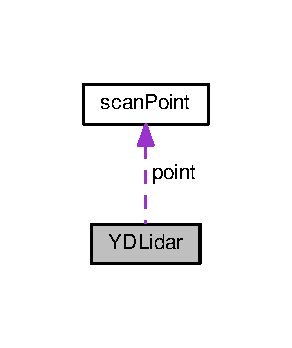
\includegraphics[width=140pt]{class_y_d_lidar__coll__graph}
\end{center}
\end{figure}
\subsection*{Public Types}
\begin{DoxyCompactItemize}
\item 
enum \{ {\bfseries S\+E\+R\+I\+A\+L\+\_\+\+B\+A\+U\+D\+R\+A\+TE} = 115200, 
{\bfseries D\+E\+F\+A\+U\+L\+T\+\_\+\+T\+I\+M\+E\+O\+UT} = 500
 \}\hypertarget{class_y_d_lidar_a93fcca770d136acd68615c077fb98fac}{}\label{class_y_d_lidar_a93fcca770d136acd68615c077fb98fac}

\end{DoxyCompactItemize}
\subsection*{Public Member Functions}
\begin{DoxyCompactItemize}
\item 
bool {\bfseries begin} (Hardware\+Serial \&serialobj, uint32\+\_\+t baudrate=S\+E\+R\+I\+A\+L\+\_\+\+B\+A\+U\+D\+R\+A\+TE)\hypertarget{class_y_d_lidar_a0c1a66b457d67fb465a82da15151bd02}{}\label{class_y_d_lidar_a0c1a66b457d67fb465a82da15151bd02}

\item 
void {\bfseries end} (void)\hypertarget{class_y_d_lidar_ab4f3a968e28e50745a86e3486570785f}{}\label{class_y_d_lidar_ab4f3a968e28e50745a86e3486570785f}

\item 
bool {\bfseries is\+Open} (void)\hypertarget{class_y_d_lidar_a114d6d4058d579e040ca2f5d4541bee9}{}\label{class_y_d_lidar_a114d6d4058d579e040ca2f5d4541bee9}

\item 
result\+\_\+t {\bfseries get\+Health} (\hyperlink{structdevice__health}{device\+\_\+health} \&health, uint32\+\_\+t timeout=D\+E\+F\+A\+U\+L\+T\+\_\+\+T\+I\+M\+E\+O\+UT)\hypertarget{class_y_d_lidar_aa85946476d601c558aea46ebf022dda3}{}\label{class_y_d_lidar_aa85946476d601c558aea46ebf022dda3}

\item 
result\+\_\+t {\bfseries get\+Device\+Info} (\hyperlink{structdevice__info}{device\+\_\+info} \&info, uint32\+\_\+t timeout=D\+E\+F\+A\+U\+L\+T\+\_\+\+T\+I\+M\+E\+O\+UT)\hypertarget{class_y_d_lidar_af39b9bbeb498209ef5d5a301e58815c7}{}\label{class_y_d_lidar_af39b9bbeb498209ef5d5a301e58815c7}

\item 
result\+\_\+t {\bfseries stop} (void)\hypertarget{class_y_d_lidar_a56dbcd8ca1e2b2b569f34189d69263a2}{}\label{class_y_d_lidar_a56dbcd8ca1e2b2b569f34189d69263a2}

\item 
result\+\_\+t {\bfseries start\+Scan} (bool force=false, uint32\+\_\+t timeout=D\+E\+F\+A\+U\+L\+T\+\_\+\+T\+I\+M\+E\+O\+UT $\ast$2)\hypertarget{class_y_d_lidar_ab94a06ee3862b4100a97c0d25dce88b5}{}\label{class_y_d_lidar_ab94a06ee3862b4100a97c0d25dce88b5}

\item 
result\+\_\+t {\bfseries wait\+Scan\+Dot} (uint32\+\_\+t timeout=D\+E\+F\+A\+U\+L\+T\+\_\+\+T\+I\+M\+E\+O\+UT)\hypertarget{class_y_d_lidar_ac4504ab865582884e27ba181acea6e10}{}\label{class_y_d_lidar_ac4504ab865582884e27ba181acea6e10}

\item 
const \hyperlink{structscan_point}{scan\+Point} \& {\bfseries get\+Current\+Scan\+Point} (void)\hypertarget{class_y_d_lidar_a704a5a434bb3022c9f169ab74ad90898}{}\label{class_y_d_lidar_a704a5a434bb3022c9f169ab74ad90898}

\end{DoxyCompactItemize}
\subsection*{Protected Member Functions}
\begin{DoxyCompactItemize}
\item 
result\+\_\+t {\bfseries send\+Command} (uint8\+\_\+t cmd, const void $\ast$payload=N\+U\+LL, size\+\_\+t payloadsize=0)\hypertarget{class_y_d_lidar_a440f59fce948f0fe000d8eee48d561c3}{}\label{class_y_d_lidar_a440f59fce948f0fe000d8eee48d561c3}

\item 
result\+\_\+t {\bfseries wait\+Response\+Header} (\hyperlink{structlidar__ans__header}{lidar\+\_\+ans\+\_\+header} $\ast$header, uint32\+\_\+t timeout=D\+E\+F\+A\+U\+L\+T\+\_\+\+T\+I\+M\+E\+O\+UT)\hypertarget{class_y_d_lidar_a05781f62737fead3f02990dfb08aadb5}{}\label{class_y_d_lidar_a05781f62737fead3f02990dfb08aadb5}

\end{DoxyCompactItemize}
\subsection*{Protected Attributes}
\begin{DoxyCompactItemize}
\item 
Hardware\+Serial $\ast$ {\bfseries \+\_\+bined\+\_\+serialdev}\hypertarget{class_y_d_lidar_aaf9925e4f8109c6b52cbd0d61df274c7}{}\label{class_y_d_lidar_aaf9925e4f8109c6b52cbd0d61df274c7}

\item 
\hyperlink{structscan_point}{scan\+Point} {\bfseries point}\hypertarget{class_y_d_lidar_aa6104f0063758211b29f7dece4e158d9}{}\label{class_y_d_lidar_aa6104f0063758211b29f7dece4e158d9}

\end{DoxyCompactItemize}


The documentation for this class was generated from the following files\+:\begin{DoxyCompactItemize}
\item 
Y\+D\+Lidar.\+h\item 
Y\+D\+Lidar.\+cpp\end{DoxyCompactItemize}

%--- End generated contents ---

% Index
\backmatter
\newpage
\phantomsection
\clearemptydoublepage
\addcontentsline{toc}{chapter}{Index}
\printindex

\end{document}
